\documentclass{article}
\usepackage[
  margin=2cm,
  includefoot,
  footskip=30pt,
]{geometry}
\usepackage{color}
\usepackage{hyperref}
\usepackage{bm}
\usepackage{amsmath}
\usepackage{amsfonts}
\usepackage{graphicx}
\usepackage{natbib}

% \newcommand{\cg}{\mathcal{G}}
% \newcommand{\cp}{\mathcal{P}}
% \newcommand{\cn}{\mathcal{N}}
% \newcommand{\E}{\mathbb{E}}
% \newcommand{\reals}{\mathbf{R}}
% \newcommand{\tr}[1]{\textrm{#1}}
% \newcommand{\red}[1]{\textcolor{red}{#1}}
% \newcommand{\blue}[1]{\textcolor{blue}{#1}}
% \newcommand{\todo}[1][]{\textcolor{red}{TODO: }\textcolor{blue}{#1}}

\title{Reconstructing Cancer Phylogeny Using Distance-based Phylogenetic Tree-Building Algorithms }
% \subtitle{BIOMATH 211: Project proposal (Winter 2023)}
\author{Helena Winata}
\date{\today}

\begin{document}
\maketitle

\section{Introduction}
Cancer is characterized by the ongoing accumulation of somatic mutations, providing selective advantages that may lead to dysregulated cellular proliferation. The mechanism at which the cancer genome accumulates and select for mutations follows a Darwinian process, resulting in clonal expansions of progressively more aberrant and fit phenotypes \cite{Tarabichi2021,Liu2020}. This allow cancers to adapt to various environmental challenges, such as treatment and metastasis. Reconstructing tumor evolution allows us to understand key events that drive cancer progression and patterns of mutation co-occurrence within clones. These evolutionary features guide our understanding of fundamental mechanisms that lead to disease lethality. 

\subsection{Comparing Cancer and Species Phylogeny}
Subclonal reconstruction (SRC) is an emerging field of caner reserach that focuses on the inference of cancer phylogeny from DNA sequencing data. Comparing cancer evolution to the more established field of species evolution can help identify transferable algorithms to accelerate advancements in SRC. Despite following similar underlying evolutionary biology principles, computational methods differ significantly between cancer and species evolution studies due to the nature of the data and biological questions of interest. SRC utilizes genetic data from a patient to infer subpopulations of cancer cells (clones) and the ancestral relationships between each of them \cite{Liu2020,phyloWGS,pyclone}. These clones are typically represented by their cellular prevalence (CP), and set of unique mutations. In contrast, species phylogeny infer evolutionary relationships between individuals based on matching molecular sequence. Both analyses aims to build a graphical representation of how clones or individuals are related hierarchically.

\subsection{Current Methods}
The most widely used methods to recontruct tumor evolution for a tumor from bulk DNA sequencing utilizes stochastic-search algorithms \cite{phyloWGS,pyclone}. For instance, phyloWGS uses Monte Carlo Markov Chains (MCMC) to traverse a Bayesian model space defined by tree topologies and subclone frequencies generated from a Dirichlet distribution \cite{phyloWGS}. The Dirichlet distribution is a multivariate probability distribution that models proportion over a number of fixed categories, and is a conjugate prior to the multinomial likelihood function, which simplifies the posterior distribution calculations. However, as tumor subclonal structure increases in complexity, the model space grows exponentially, and stochastic-search algorithms become computationally intractable. For instance, recent benchmarking studies have revealed that many methods fail to reconstruct clone trees for data with as few as ten subclones \cite{pairtree}. 

This project aims to explore the application of distance-based tree-building algortithms in an effort to search for alternative methods for SRC. Simulated datasets will be used to enable quantitative evaluation of the performance of these methods in a controlled setting. Additionally, building the simulation for data generation will provide a resource that can be expanded to benchmark methods in the field.

\section{Method}
Code for data simulation and analysis are available on \href{https://github.com/whelena/BIOMATH211_Cancer-Phylogeny}{GitHub}.

\subsection{Data Simulation}
\begin{figure}[!ht]\centering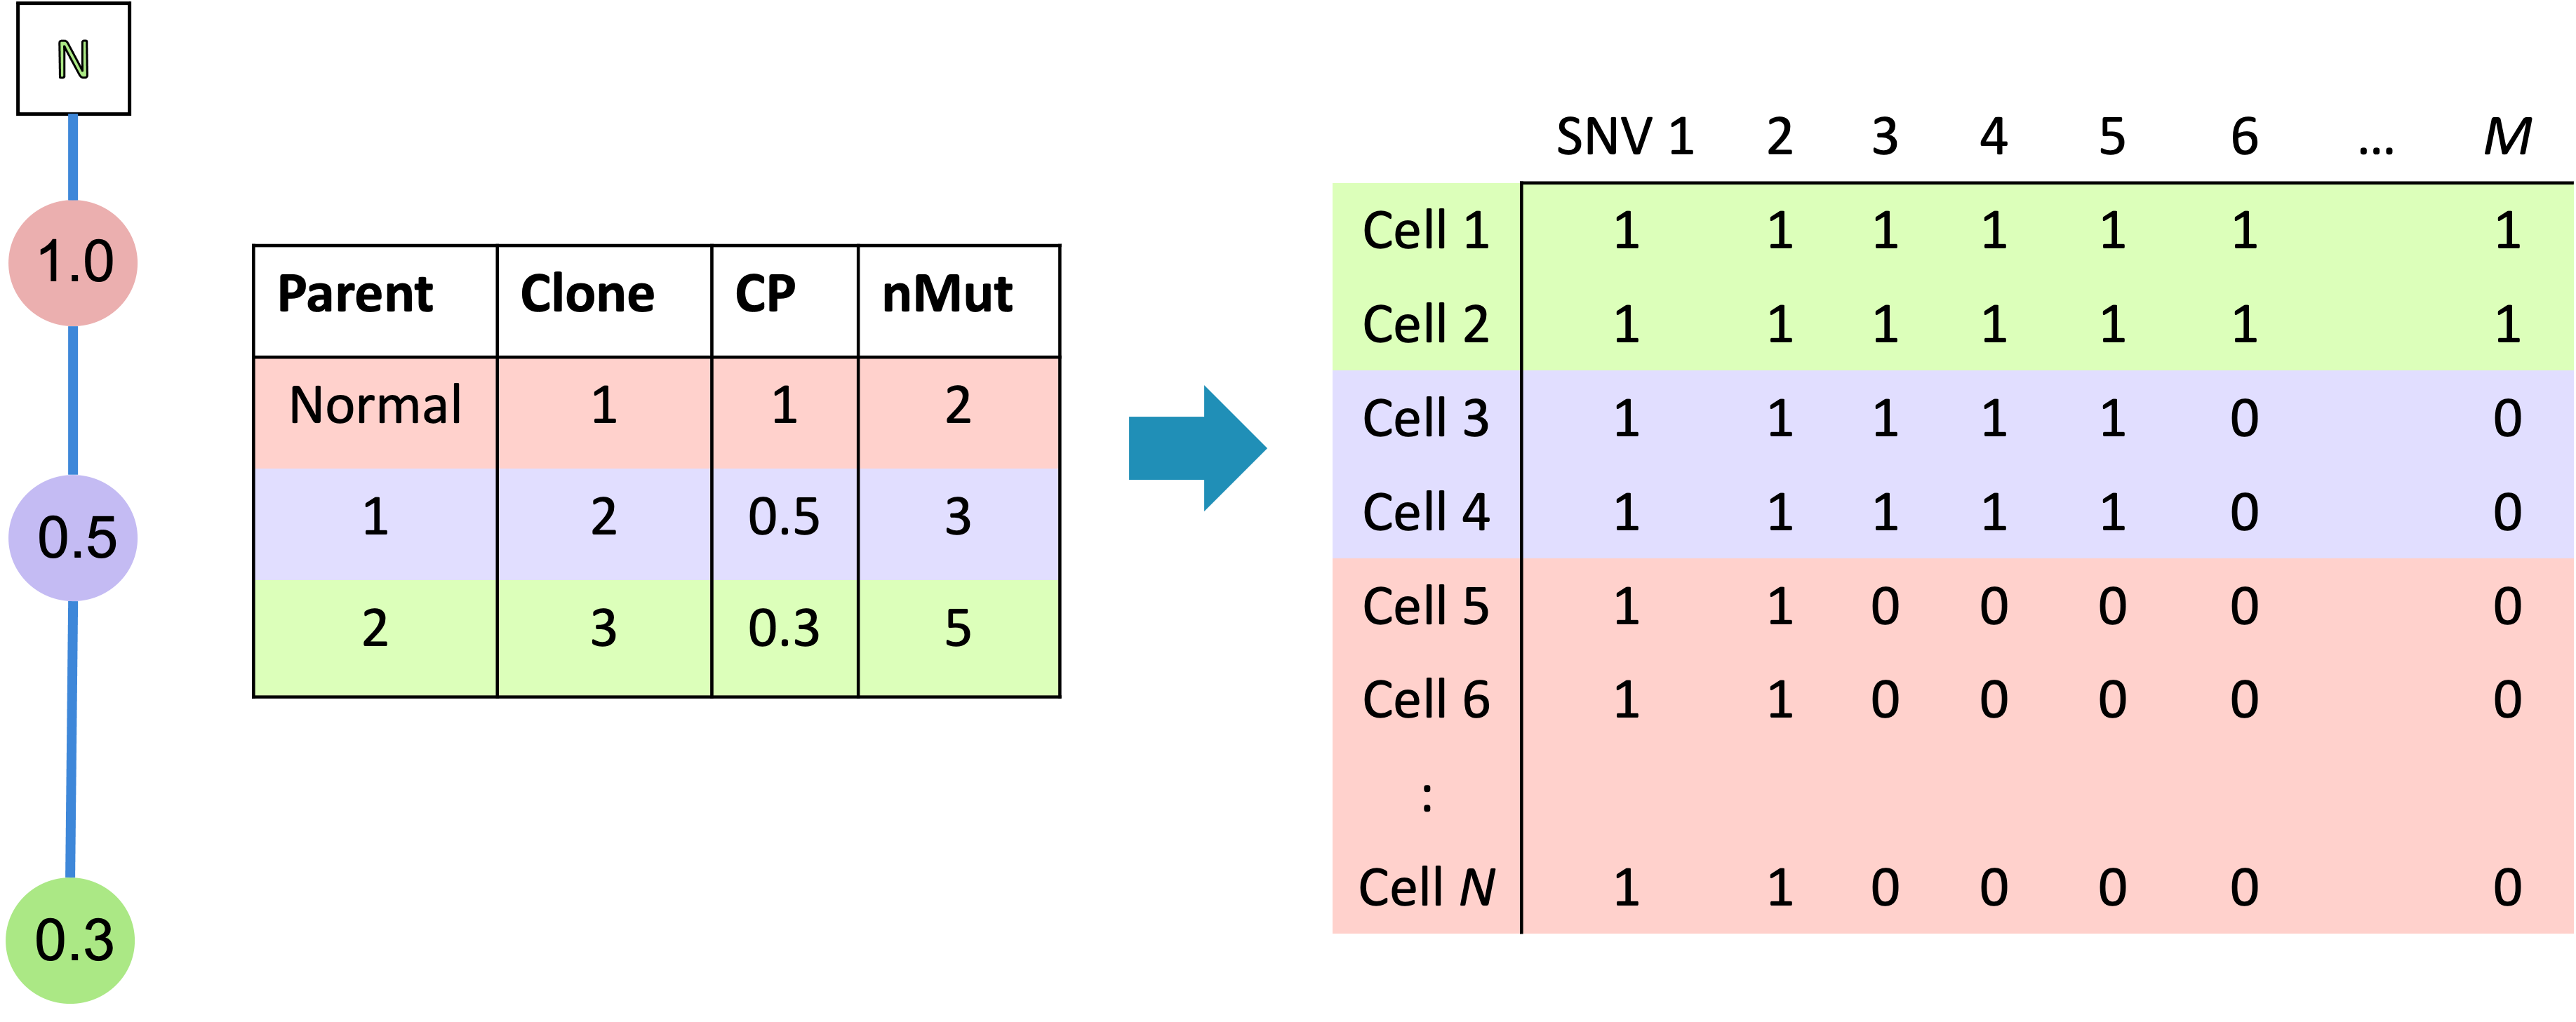
\includegraphics[width=0.8\textwidth]{fig/sim.png}
    \caption{\label{fig:sim} Simulated datasets showing the tree topology, phylogeny table and cell mutation profile (left to right). N denotes the normal, which has no mutations.}
\end{figure}
    
First, cellular prevalences (CP) for a number of clones are simulated through nested sampling from a uniform distribution between 0 and 1. All phylogenies are simulated to be linear (no branching). Similarly, nested sampling is done to assign the number of unique mutations to each clone, such that the total sum up to the given parameter. The number of cell containing the unique mutations for each clone is determined by the simulated CP (equation \ref{eq:cp}), and cells in each clone inherits all the unique mutation of its parent clone. For instance, in figure \ref{fig:sim}, the green cells (clone 3) inherited all the mutations from subsequenct clones. To generate the mutation profile for each cell, each mutation modelled as a Bernoulli trial with a noise parameter that models sequencing and mutation detection errors  (equation \ref{eq:mp}). This results in mutation vestor ,$Y_i$ for each cell, where the proportion of cells containing a mutaion, $CP_j$ is shown in equantion \ref{eq:cp}. Overall, 81 single cell data were simulated with different combinations of these following parameters: number of clones ($K$): 3, 5, 20; number of cells ($N$):  50, 100, 200; number of mutations ($M$): 50, 100, 200 and noise ($\epsilon$): 0.05, 0.1, 0.2.

\begin{equation} \label{eq:cp}
    CP_j = \frac{1}{N}  \sum^N_i Y_{ij}
\end{equation}

\begin{equation} \label{eq:mp}
    Y_{ij} \sim \begin{cases}
        Bernoulli(1, 1, (1 - \epsilon)) & \text{if } i \in k \\
        Bernoulli(1, 1, \epsilon) & \text{otherwise}
        \end{cases}
\end{equation}

\subsection{Clustering and Cluster Metrics}
Tree building from simulated single cell data is done using Neighbour-Joining (NJ) on manhattan pairwise distances between individual cells. Clones were then recovered by pruning the tree, using the number of clones, $K$, as the desired number of clusters.

To quantitatively evaluate the clusters generated from the NJ trees, the adjusted rand index (ARI) and average silhouette width (ASW) were calculated. ARI measure the similarity between two clusterings by measuring the number of matches between cluster labels. A score of 1 indicates perfect concordance between labels, 0 indicates agreement by random chance and -1 indicates disagreement higher than expected by random chance. ASW measures the quality of clusters generated based on how well each data point fit its assigned cluster. Silhouette scores are calculated based on the distance between each cell to cells from the same cluster compared to cells from the nearest cluster. The score range from -1 to 1, where 1 indicates a well-clustered cell, and -1 indicating a mis-clustered cell. Finally, pearson's correlation were calculated for each parameter vs. metric to identify any significant linear relationship between the variables.

\section{Results and Discussion}
\begin{figure}[!ht]\centering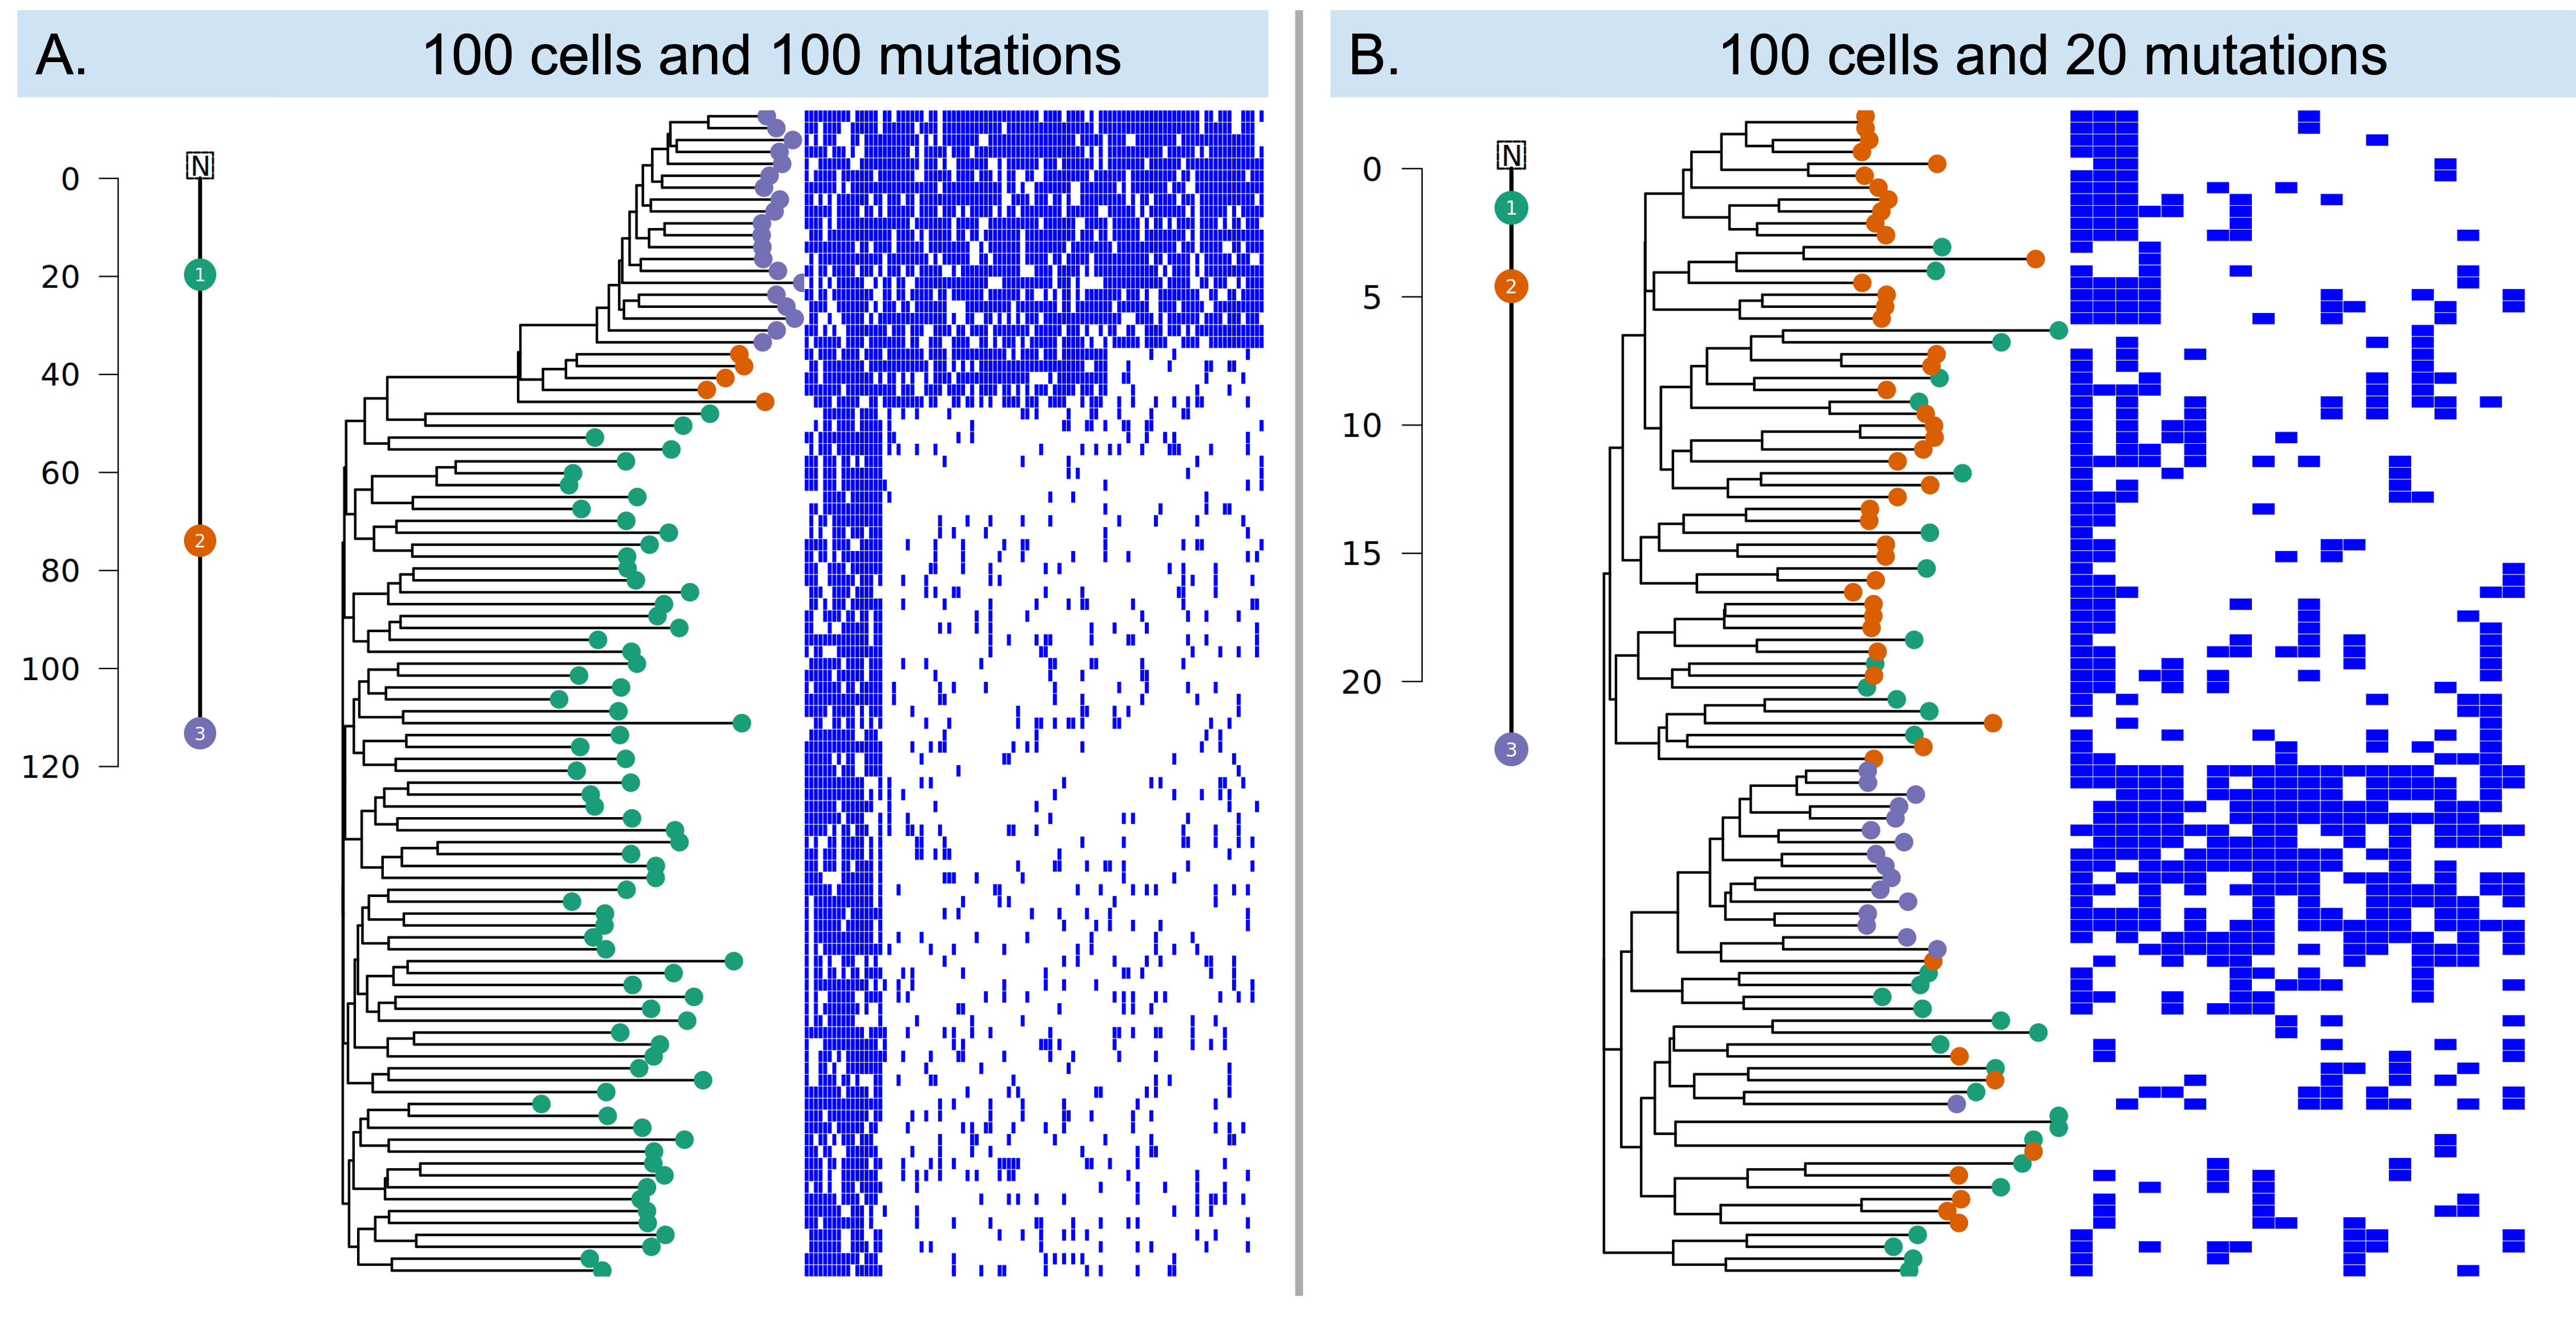
\includegraphics[width=0.8\textwidth]{fig/result.png}
\caption{\label{fig:result} Figure showing two examples of the simulated phylogeny, dendrogram of cells and heatmap of simulated mutations. Leaf nodes are coloured based on their true clone labels. Both datasets are simulated for 3 clones with noise = 0.2, with other parameters specified in the figure. The ASW scores for dataset A and B are 0.64 and 0.11, respectively. The ARI scores for dataset A and B are 0.92 and 0.23.}      
\end{figure}


Figure \ref{fig:result} shows the distribution of true clone labels across the NJ tree tips. This reveal how well the NJ mehthod was able to distinguish cells from different clones based on their mutation profiles. To supplement this with quantitative evaluation, ARI and ASW scores are calculated to measure conordance between true and predicted clone labels as well as how tight or well-separated the clusters are.

\begin{figure}[!ht]\centering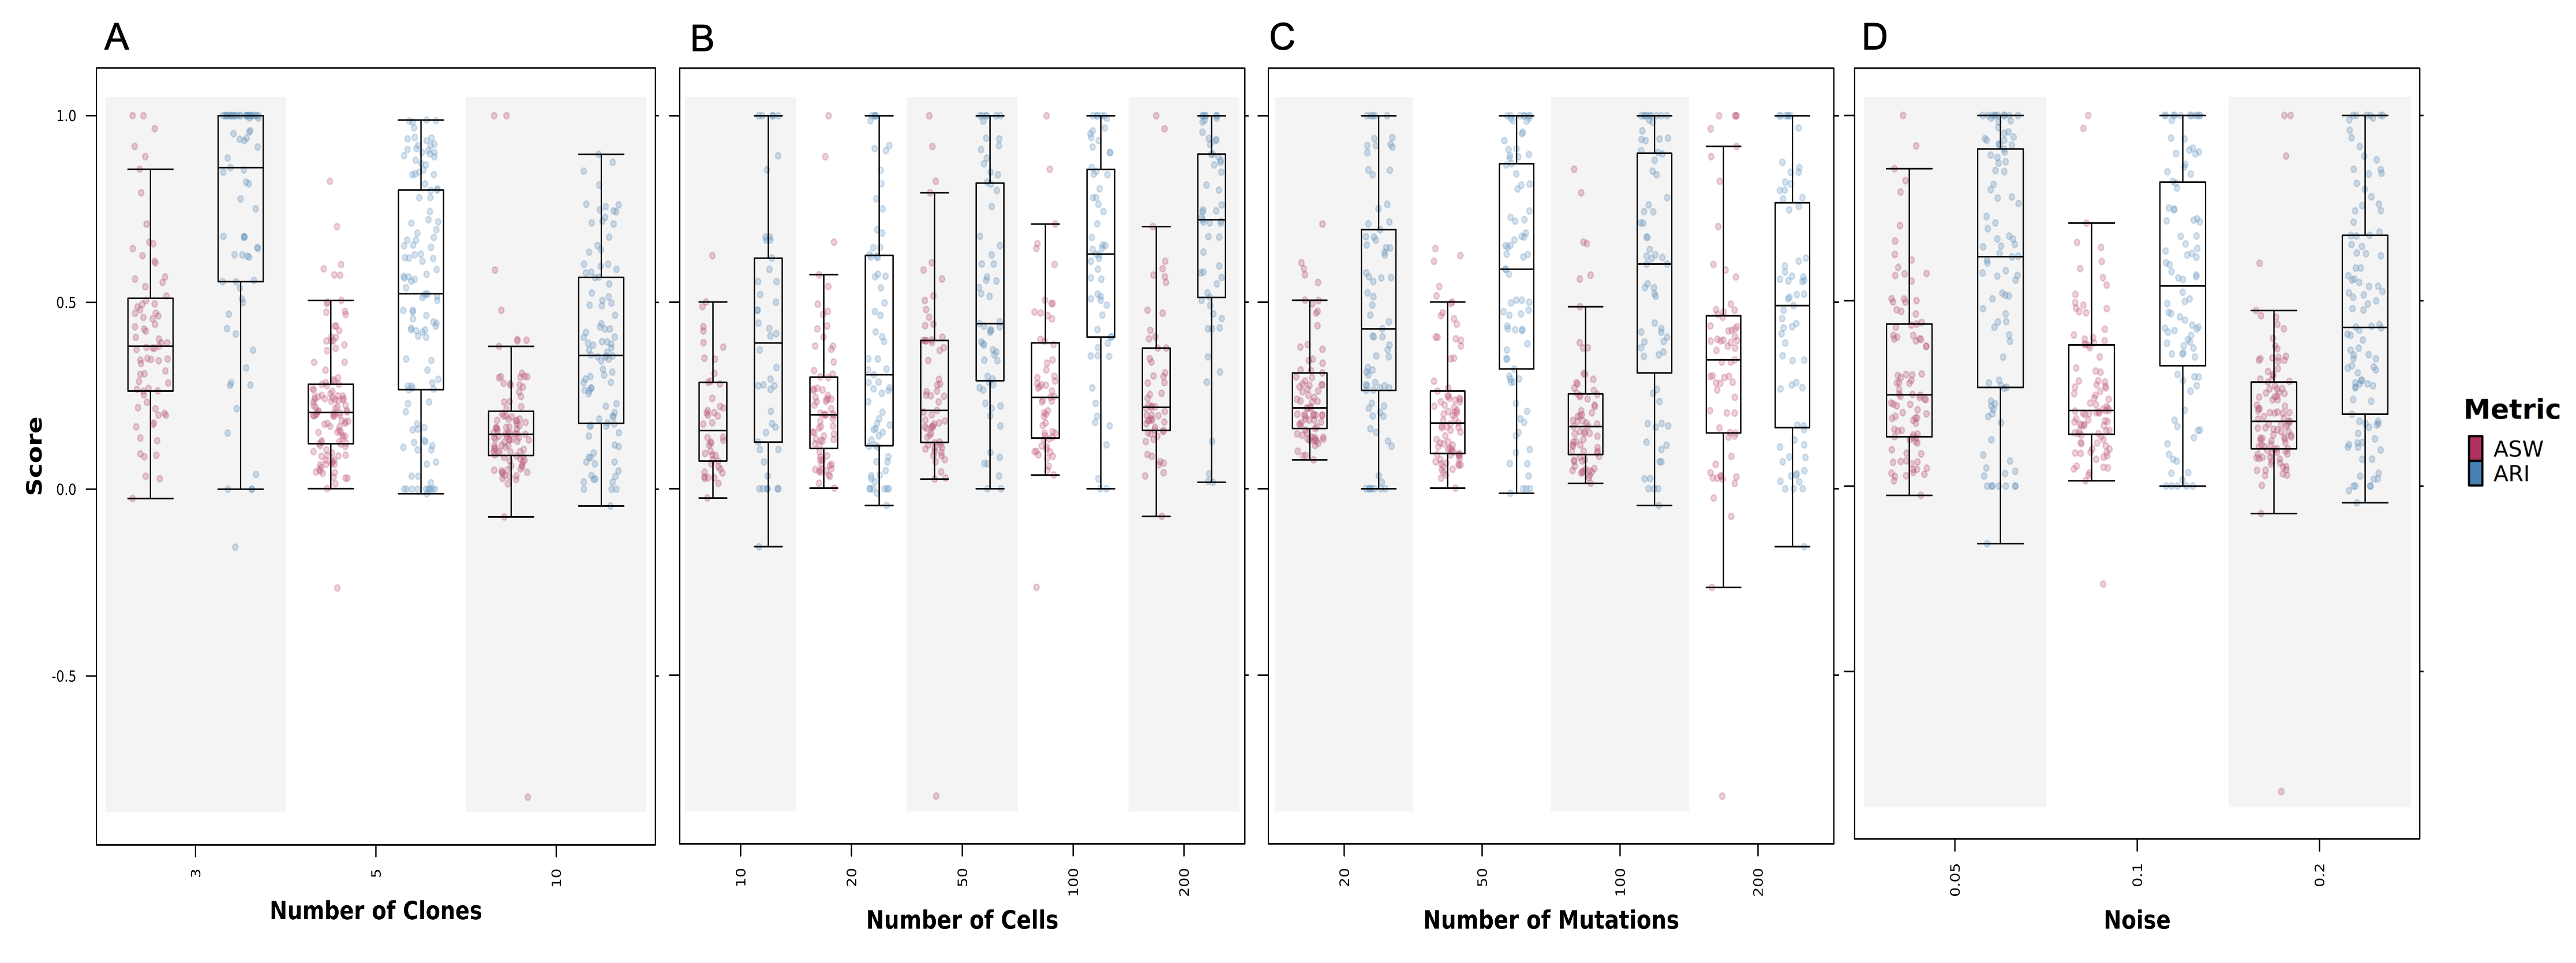
\includegraphics[width=0.8\textwidth]{fig/stat.png}
    \caption{\label{fig:stat} Distribution of cluster scoring metrics for eeach simulated dataset.}      
\end{figure}

Figure \ref{fig:stat} shows the distribution of ASW and ARI scores for each parameter: clones, separated by the number of clones, cells, mutations and noise. The number of clones, mutations and noise are significantly correlated with ASW scores, with a pearscon's coefficient of -0.38, 0.18, -0.19, and p-value of $2.31E-11$, 0.002, $8.57E-4$, respectively. For ARI scores, the number of clones, cells and noise are all negatively correlated with scores of -0.39, 0.33, -0.15 and p-value of $3.16E-12$, $3.89E-9$, 0.008, respectively.

Significant negative correlation between ASW with number of clones, mutations and noise is expected. Increasing the number of clones reduces the inter-cluster distances, while increasing noise obscures the boundaries between clusters. Similarly, negative correlation was found between ARI scores and number of clones and noise. Alternatively, the number of mutations show a significant positive correlation with ASW, while the number of clones correlate significantly with ARI. The correlation coefficient and p-value for the relationship between number of cells and ASW are 0.11 and 0052, respectively. Taking both metrics into account, expanding the dataset by sequencing more cells or samples are likely to be more effective than sequencing more sites or mutations. Number of clones have the largest correlation coefficient magnitude and smallest p-value for both ASW and ARI scores. This provides strong evidence that increasing the number of clones negatively impacts the ability to resolve distinct clones, likely due to the overlaps in cellular prevalences of the clones. By restricting the simulation to non-branching trees, adding more clones directly decreases the difference between clone CP. This observation needs to be validated in branching trees.

The field of SRC lacks standardization and benchmarking studies due to the complexity and novelty of the analysis. Quantification of how properties of the data, such as mutation calls and read depth, affect the accuracy of SRC was only recently published \cite{Liu2020,Tarabichi2021}. Simulating datasets with know ground truth, and defining quantifiable metrics that measures the accuracy are a few of the limitations faced by the field. Findings derived from simple simulations and methods, such as presented here, can provide valuable insights to guide future research directions.

\section{Conclusion}
Single cell DNA sequencing is not yet a standard practivce for cancer SRC. However, as sequencing costs drop and novel bioinformatic tools specialized for this data type emerges, single-cell DNA sequencing will enable the study of tumor evolution in unparalleled detail. Despite the limited scope of the current simulated dataset, results show some indication on factors affecting the precision and accuracy of SRC using single cell sequencing data. Single cell studies typically deal with many samples/cells, which is incompatible and intractable with current methods. Therefore, investigating transferable methods from a similar, more advaced field of species phylogeny can inspire novel methods in SRC. The application of NJ algorithm on reconstructing cancer phylogeny shown here is an example of that effort. The simulation framework developed here can be adapted to simulate more complex tumor phylogenies including branched topologies, and multi sample data that represents tumor samples taken from across spatial or temporal space. This will allow further exploration of the utility and limitations of NJ and other phylogenetic methods in SRC. Furthermore, simulating both bulk and single cell data, and comparing the reconstructions will allow further benchmarking of novel methods or to evaluate the utility of single cell sequencing for SRC.


\pagebreak

\bibliographystyle{unsrt}
\bibliography{references} 

\end{document}
